\documentclass[tikz]{standalone}

\colorlet{FilledSurface}{blue!20}
\colorlet{FilledSurfaceGroupOne}{blue!20}
\colorlet{FilledSurfaceGroupTwo}{red!20}
\colorlet{FilledSurfaceGroupThree}{green!20}
\colorlet{FilledSurfaceGroupFour}{magenta!20}
\colorlet{FormulaBackground}{green!10}
\colorlet{FormulaFrame}{green}


\usetikzlibrary{calc, angles}

\begin{document}
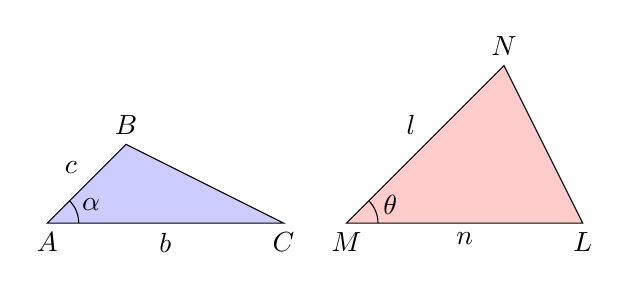
\begin{tikzpicture}

    \coordinate (A) at (0,0);
    \coordinate (B) at (1,1);
    \coordinate (C) at (3,0);

    \coordinate (M) at (3.8,0);
    \coordinate (N) at (5.8,2);
    \coordinate (L) at (6.8,0);

    \draw [fill=FilledSurfaceGroupOne] (A) node [below]{$A$}
    -- node [above left] {$c$} (B) node [above]{$B$}
    -- (C) node [below]{$C$}
    -- node [below] {$b$}  cycle;

    \draw [fill=FilledSurfaceGroupTwo] (M) node [below]{$M$}
    -- node [above left] {$l$} (N) node [above]{$N$}
    -- (L) node [below]{$L$}
    -- node [below] {$n$} cycle;

    \path pic [draw, angle eccentricity = 1.5, angle radius = 4mm, pic text={$\alpha$}] {angle = C--A--B};
    \path pic [draw, angle eccentricity = 1.5, angle radius = 4mm, pic text={$\theta$}] {angle = L--M--N};

\end{tikzpicture}
\end{document}

